\documentclass{oblivoir}
\usepackage{amsmath,amssymb,amsthm,kotex,mdframed,paralist,kswrapfig}

\newcounter{num}
\newcommand{\theo}[1]
{\bigskip\noindent\refstepcounter{num}\textbf{정리 \arabic{num}) #1}\par}
\newcommand{\prob}[1]
{\bigskip\noindent\refstepcounter{num}\textbf{문제 \arabic{num}) #1}\par}

\renewcommand{\figurename}{그림}

\newcommand\ov[2]{\ensuremath{\overline{#1#2}}}

\begin{document}

\title{현빈 17 : 메넬라우스의 정리, 체바의 정리}
\author{}
\date{\today}
\maketitle
\newpage

%
\theo{메넬라우스의 정리}\label{menelaus}
그림 1과 같이 한 직선 \(l\)이 \(\triangle ABC\)의 세 변 \ov BC, \ov CA, \ov AB(또는 그 연장선)를 잘랐을 때의 교점이 각각 \(D\), \(E\),\(F\)이면
\[
\frac{\ov AF}{\ov FB}\cdot\frac{\ov BD}{\ov DC}\cdot\frac{\ov CE}{\ov EA}=1
\]
이다.

\begin{figure}[b]
\centering
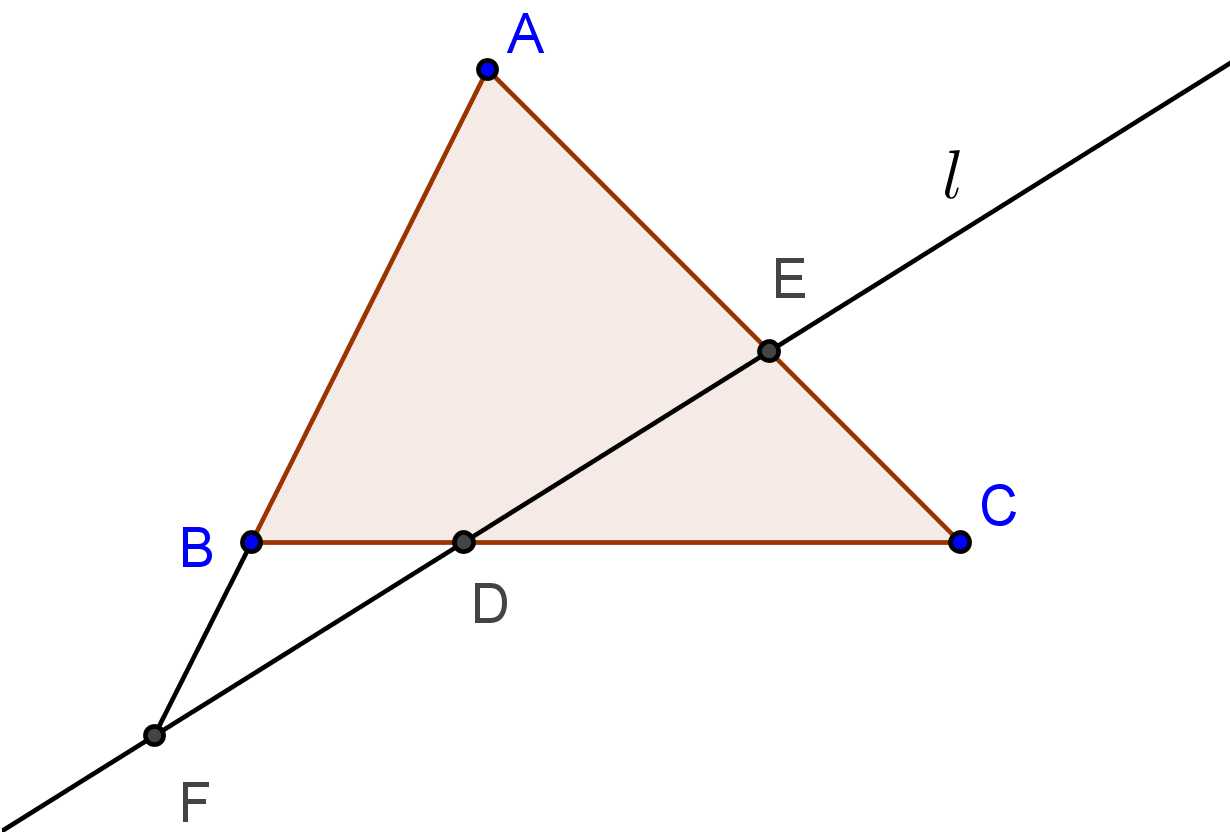
\includegraphics[width=0.5\textwidth]{menelaus}
\caption{메넬라우스의 정리}
\end{figure}

\bigskip
\begin{mdframed}
증명 : 
\vspace{0.1\textheight}
\end{mdframed}

%
\theo{메넬라우스의 정리의 역}\label{c-menelaus}
\(\triangle ABC\)의 세 변 \ov BC, \ov CA, \ov AB(또는 그 연장선) 위에서
\[
\frac{\ov AF}{\ov FB}\cdot\frac{\ov BD}{\ov DC}\cdot\frac{\ov CE}{\ov EA}=1
\]
이 되게 각각 \(D\), \(E\), \(F\)를 취하면 \(D\), \(E\), \(F\)는 한 직선 위에 있다.

\bigskip
\begin{mdframed}
증명 : 
\vspace{0.1\textheight}
\end{mdframed}
\newpage

%
\theo{체바의 정리}\label{menelaus}
그림 2과 같이 \(\triangle ABC\)의 세 꼭짓점과 그 대변(또는 그 연장선) 위의 한 점 \(D\), \(E\), \(F\)를 연결하여 \ov AD, \ov BE, \ov CF가 한 점 \(P\)에서 만나면
\[
\frac{\ov AF}{\ov FB}\cdot\frac{\ov BD}{\ov DC}\cdot\frac{\ov CE}{\ov EA}=1
\]
이다.

\bigskip
\begin{mdframed}
증명 : 
\vspace{0.1\textheight}
\end{mdframed}

\begin{figure}[b]
\centering
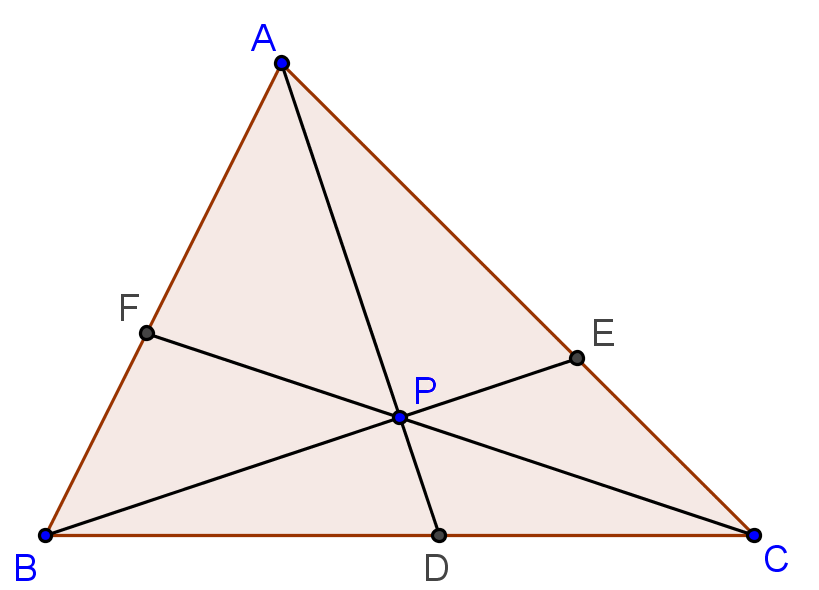
\includegraphics[width=0.5\textwidth]{ceva}
\caption{체바의 정리}
\end{figure}

%
\theo{체바의 정리의 역}\label{c-menelaus}
\(\triangle ABC\)의 세 변 \ov BC, \ov CA, \ov AB(또는 그 연장선) 위에서
\[
\frac{\ov AF}{\ov FB}\cdot\frac{\ov BD}{\ov DC}\cdot\frac{\ov CE}{\ov EA}=1
\]
이 되게 각각 \(D\), \(E\), \(F\)를 취하면 \(D\), \(E\), \(F\)는 한 직선 위에 있다.

\bigskip
\begin{mdframed}
증명 : 
\vspace{0.1\textheight}
\end{mdframed}
\newpage

%
\kswrapfig[Pos=r]{01}{
\textbf{문제 1)}\\
\ov BD=4, \ov CD=8, \ov AE=9, \ov CE=3, \ov AB=10 일 때, \ov BF의 값을 구하시오.}
%\begin{figure}[h]
%\centering
%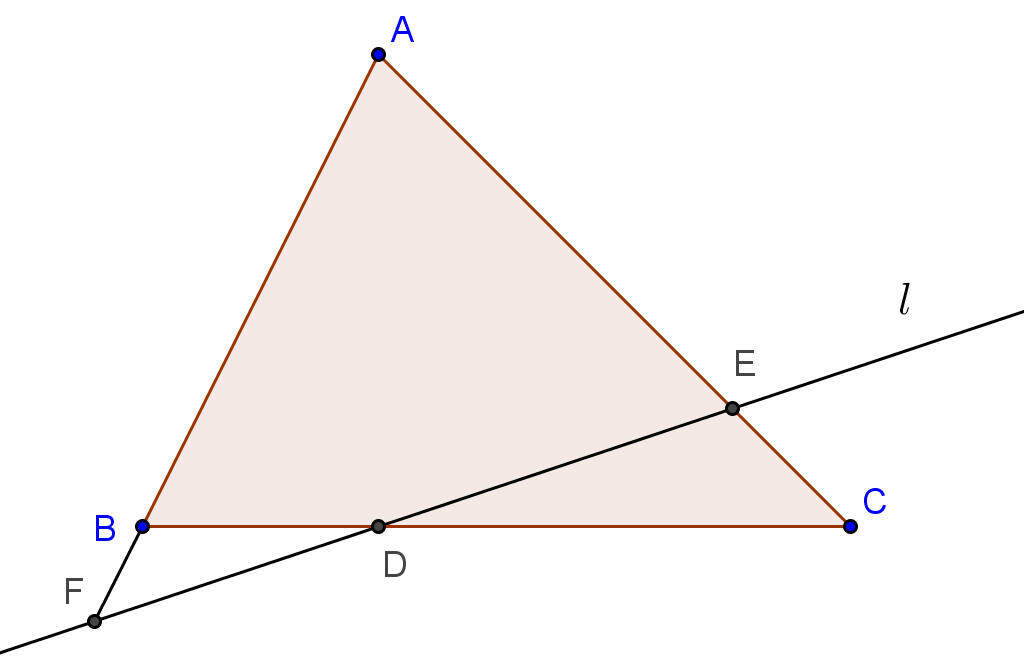
\includegraphics[width=0.5\textwidth]{01}
%\end{figure}

%
\kswrapfig[Pos=r]{02}{
\textbf{문제 2)}\\
\ov BD=6, \ov CD=3, \ov AE=6, \ov CE=2, \ov BF=3 일 때, \ov AF의 값을 구하시오.}

%
\kswrapfig[Pos=r]{03}{
\textbf{문제 3)}\\
오른쪽 그림의 삼각형 \(ABC\)에서 \(\overline{AB}=5\), \(\overline{BF}=4\), \ov CF=3이다. 
\ov AD\::\:\ov CD=3\::\:2일 때, \(\frac{\overline{AG}}{\overline{GF}}\)의 값은?
}

%
\kswrapfig[Pos=r]{04}{
\textbf{문제 4)}\\
오른쪽 그림의 사다리꼴 \(ABCD\)에서 \(\overline{BC}=12\), \(\overline{DE}=4\), \ov AB=10이다. 
\ov DF의 값은?
}




\end{document}